\chapter{Experiment}
\label{cha:Experiment}
This section describes the experiments conducted in order to be able, to answer the defined research questions. In the previous chapter (\ref{cha:Approach}) the general methodology used technologies got described, to gain an understanding of the implementation and its components. Based on this knowledge and implementation, some experiments got conducted, that provide interesting results and meaningful insights into this approach of neural audio synthesis. For the purpose of this thesis, some research questions have been defined, for which the following experiments, deliver the answers, which get discussed later on when showing the results.\\

\noindent Those research question are defined as the following:

\begin{itemize}
    \item \textbf{Is it possible to create novel sounds based on the characteristics of two instruments, by using ML technologies such as convolutional neural networks?}

    \item How do the pre processing steps influence the quality of the training, but also the quality of the output?

    \item How does the configuration/composition of a neural network influence the quality of the output?

    \item What are the information that are learnt from the neural network?

    \item By using audio spectrograms, are they suited best to achieve this task?
\end{itemize}

In the last section, when describing the different technologies, it has been mentioned, that they can be parameterized in order to influence the outcome of this work. Furthermore some additional steps can be introduced that have a significant impact on the result. This section therefore describes, how the proposed methods were utilized, in order to answer the above mentioned questions. Furthermore those experiments, should deliver some interesting insights, on how different configurations influence the workflow but also the final result being a synthesized audio. Those experiments span almost every stage from the pre-processing until post-processing. 

\section{Implementation Environment}
In the previous chapter it has already been mentioned, that this approach is developed in python using specific libraries. To shortly mention, for pre- and post-processing the python audio-library \textit{librosa}\cite{brian_mcfee_2022_6097378} has been chosen, as it provides all necessary functionalities that are needed for the approach and experiment. For all steps regarding the neural network model such as configuration, training, inference etc., \textit{PyTorch}\cite{paszke2019pytorch} has been utilized. The project though has been implemented and applied on two different machines, depending on the task that has to be done. Generally speaking, the toolchain compromised of all stages, has been developed on a local machine running python, except the training itself. 

Speaking of that, the training has been mainly performed on a remote "jupyter-notebook" that has access to high-performance GPU resources. Not at least, as in the case of training a convolutional neural network, this is a rather time and computational power-consuming task. Of course, this not only depends on the kind and complexity of the network, but also on the amount of data that is used for the training. Furthermore using GPU-acceleration means to significantly have more computation power and speed, as its applying parallelism. Using the local machine, just the CPU could be utilized for training, which would mean that training is done sequentially and thus significantly slower while the local machine has to be awake constantly. For the training on the remote instance, the pre-processing also gets done there as the data is directly loaded there. 
As just the training is performed remotely, all other steps, including the evaluation towards audio (re)synthesis having the trained model, gets again done locally. Not at least, as no time-consuming tasks have to be made, but also as its more convenient, as the remote service is not always accessible.


\section{Training}
The training, as mentioned previously, gets performed on a remote "jupyter notebook"-service with access to a GPU. As outlined in the previous chapter, for the whole experiments, the NSynth data set proposed by \textit{Engel et al.}\cite{Engel2017}, gets used. As is well known this dataset is already split into a training, validation and test part. For the training on the remote notebook, the training and validation data set will therefore be used, which in order also get pre-processed there. As a side note, in the beginning of the project, the training was just held locally, with a small subset of the already small test set (mostly of one instrument). This was just done to make a low-level proof that the autoencoder model can produce meaningful results. 

\subsection{Training configuration}
To take a closer look onto the training process, this one consists of several important stages and components. First of all the PyTorch-model, defined as a class, gets initialized. As an metric is needed, to measure the error of the output, the mean squared error (MSE) gets utilized. This error metric calculates the difference between all values of the desired and actual output, squares them, and takes the average over all. Furthermore to optimize the network, as explained before, the Adam optimizer gets applied, in which the (starting) learning rate, but also the weight decay gets defined. The right learning rate depends here heavily on the amount of training data but also complexity of model. In the case of this work, this means it is in the range between $1e-5$ to $1e-7$. In chapter \ref{cha:Approach} it got also mentioned, that a technique to minimize the the learning rate, during the training process gets utilized. This function called \texttt{torch.optim.lr\_scheduler.ReduceLROnPlateau(...)} reduces the learning rate, by a given factor, if within a certain patience period (epochs) no optimization gets detected. This method, improves the training process as further convergence can be achieved. Of course for the training process, the pre-processed training and validation data set has to be loaded. To mentioned, the pre-processed data gets calculated and stored on disk, in advance, to not always have to run through it. for the training it therefore gets loaded and brought into the desired shape for the corresponding model. This shape gets varied throughout the experiments, to observe its impact on the training process but also quality of the output. As this also depends on the chosen network, this gets described later on in this chapter. For the sake of training, this gets done with the training dataset, as well as for the validation dataset, as after each epoch the model gets evaluated on a held out validation set, to check the error on never seen data.
The data in the right shape, has to be converted to a tensor and in further notice, to a (custom) dataset object. Finally a so called "DataLoader" has to be initialized, either for the training but also for the validation. In this DataLoader the batch size can be specified, whitch is an important parameter regarding the training. Throughout a few batch sizes, have been tried out, whereas in the end, the prefered batch size was 32. This means that the input data, gets portioned in equally sized chunks of 32 tensors, that get fed into the network at once. Further on it can be set, that after each training epoch, the dataset gets shuffled. Setting this to true, the samples in the batches are in a different order and constellation. Otherwise, the batches consist always of the same data in the same order. Throughout the experiments, this setting was proven to be advantageous regarding the convergence of the model, as the error could be more minimized (see chapter \ref{cha:Results}).

\subsection{Training Execution}
Having the configured dataloaders, which are also iterables, it is possible to iterate over the batches of the dataset. Before the training begins, a number of epochs has to be set, which defines how often the training should be performed on the whole dataset. In advance it cannot be said, how many epochs are needed, therefore a preferably big number gets chosen e.g. 1000. To clarify, the training never runs until the final epochs, as it get stopped at a point, where the result is sufficient (more on that shortly). In each iteration, the corresponding batch of data will get input into the network with a forward pass which calculates an output. This output gets compared to the desired value, which is in this case the same as the input, and further on the error gets calculated. Further on the gradients get computed and optimization via parameter update is done. The loss value gets added up, and after all batches are done, the average loss gets computed, to show the progress. 

After all train batches have ran through and optimization is done, the model gets validated using the held out validation set. This one is also equally batched, and runs through the same process, except there is no optimization. Here there error is just calculated to see, how the model performs on data that is not used for training and therfore never seen before by the network. This technique helps to prevent to overfit the training data, which would be signalized through an increasing validation error despite training error gets smaller. Having the validation error after each epoch, this value gets used for the learning rate scheduler to decrease the learning rate if the error does not decrease in a certain period. 

 To ensure to have a sufficient trained network, the error scores get observed periodically. If the validation score does not improve more, i.e. the network convergence stagnates, and is sufficient, the training gets stopped. Important to know that after each training iteration, which is also called epoch, the state of the model gets saved, for further use. As also the scores for each model state is known, it is therefore possible to determine the best model, having the lowest MSE-score on the validation data. This one then gets further tested and analyzed towards the applicability for audio (re)synthesis. Those further steps, which do not involve training, as well as the pre-processing regarding the evaluation data, get performed locally. 

 
\section{Initial Experiments}
In the beginning of this project, initial experiments, were done in order to make a very basic proof of concept implementation. Like mentioned before, those implementations, where entirely held on the local machine, not at least as there was no access to GPU-accelerated training. This was also possible, due to just taking a small subset of the test dataset. Of this test dataset, samples of one instrument (\textit{keyboard\_synthetic}) were taken out, and considered for test-wise training.

\subsection{Whole Spectrograms as Input}

\subsubsection{Pre-processing}
For the first experiments, all the samples of the subset, have been converted to log-magnitude spectrograms as a whole. As already known, those samples have all the same length of 4 seconds. Some samples are padded with zeros, as those do not contain audio data over the full length. As parameters for the STFT \texttt{n\_fft} of 512 and \texttt{hop\_length} of 256 got chosen. This configuration results in spectrograms having 257 frequency bins with a resolution of 31,25 Hz. Regarding the time-resolution it can be said, that each frequency vector represents 16 milliseconds of the original signal with a 50\% overlap. This procedure resulted in spectrograms with a dimension of 257x250. 

\subsubsection{Model and training}
As the spectrograms can be seen as grey-scale images, and thus 2D-Convolutions got applied, a third dimension got added resulting in 257x250x1 spectrograms.  Finally to form a dataset ready for training, all the spectrograms of the mentioned subset got concatenated to a 4D-array, which was converted into a tensor and subsequently into a dataset. The following training, was performed on 80\% of this subset, whereas the other 20\% were used for evaluation. Regarding the duration of the training, this was held for a short time (~20 epochs).

To also mention the model configuration, this consists of 4 convolutional layers in the encoder including ReLU activation and batch normalization. The decoder part has therefore also 4 layers, which contain respective convolutional-transpose layers with also ReLU and batch normalization except the very last layer. Another important detail is, because of the shape of the input, that the number of input channels has to be 1. Throughout the network, this parameter gets varied, whereas in the first layer an expansion is being made to 225, subsequently in the second to 256 output channels. To the innermost layer it gets again reduced to 100. In the decoder part, again an expansion is being made, whereas at the end it gets reduced to 1 channel again, in order to match the input size. This configuration is the same for this and the following experiment.

\subsubsection{Testing/Evaluation}
Regarding the evaluation of this first model, it has been tested out on the remaining 20\% of the small subset. These first experiments, consisted just of evaluating the outcome of the decoder, by passing single spectrograms through the network. By this, the ability of the network to recreate audio spectrograms got proven, which further on serves as a base for the next experiments. Regarding the final outcoming sounds, the original preserved phase information was reused to recreate audios.

\subsection{Framed Spectrograms as Input}
In the previous initial experiment, the samples from the NSynth dataset have been taken as a whole for the experiment. It has been mentioned, that all samples are 4 seconds long, but some contain padding in order to come to the 4 seconds. As those zero-paddings are then also part of the trained that, this could affect the behaviour but also the outcome of the model. If those zero-paddings would be left out, this leads to unequal long samples, which brings the problem with it, that they cannot be used for the model. Not used at all, as the network has a fixed size of neurons at the input, which means that the input has to be in a fixed shape. Furthermore this also means, that having a fixed size of 4 seconds, the input always has to be of 4 seconds, which is not desirable. Not at least, if the system should be used in real-time applications for audio synthesis, one cannot wait to have 4 seconds of a signal, to perform audio synthesis with it. Therefore it would be desirable to perform audio synthesis on smaller "frames or chunks" of an audio signal, respective spectrogram. 

\subsubsection{Pre-processing}
This leads, to the idea to take chunks or frames of audio data that get transformed into distinct spectrograms of same size. For a start the length of those frames, gets set to 500 ms. Furthermore it got chosen, that those frames are not consecutive, but have an overlap of 50\%. This should preserve the continuity of the signal \footnote{not sure if right}. Additionally those frames get multiplied with a window function, like it is used in the STFT. Similar to the window function used in the STFT, here a Hann-window is used.  Again as those trimmed signals all are differently long, they have to get padded to a multiple of the frame size respective hop-length. This ensures to have equally long chunks of the signal. As of the windowed frames, the first and last frame don't have overlapping parts at the beginning respective end. To overcome this issue, additional zeros get added there to form one frame on each side, to get there also an overlap. In combination, having the framed and windowed signal chunks, by overlapping each again with 50\% and adding the values, this would yield the original signal again. This gets especially helpful when reconstructing the final signal in the end. 

Having those framed and windowed signal chunks, the STFT gets applied on those, having the same configuration as in the first experiment. This then leads to have multiple spectrograms for the length of 500 ms with again a frequency resolution of 31,25 Hz. Again for the training and testing, additional to the log-mag data, the phase information, reference value and name of the sample including a number to identify the frame.

\subsubsection{Model and training}
The configuration of the model is rather similar to the one used in the first setting. It has the same amount of layers on each side, despite different strides, but also different kernel-sizes got applied. Again this one has been trained on 80\% of the \textit{keyboard\_synthetic} test dataset samples. Of course the significant difference here is, that now the input data are not whole spectrograms but overlapping frames. This also means, that the amount of data has increased. When collecting the spectrograms for the dataset, the names get shuffled, in order to not have the same order. In contrast, the single frames, don't get shuffled as well not during training. Again the training has been performed over 20 epochs on the local machine.

\subsubsection{Testing/Evaluation}
For the purpose of evaluating the test score this has been done with the remaining 20\% of the samples. To evaluate the ability of the autoencoder to reconstruct spectrograms, the whole samples are used including those from the training. Here the spectrograms are provided in the order as they appear. Having all reconstructed spectrograms, the inverse STFT got applied with the preserved phase information. Resulting in the frames corresponding to every single input note, those got overlapped and added (in their right order). By this procedure the signal with the original length could be obtained and further on evaluated auditorily. For results see chapter \ref{cha:Results}. 

A step for interpolating two different sources has not been investigated here, up to these experiments. Also the embedded space also has not been evaluated so far but will be subject of further experiments.

\section{Experiments single frequency vectors}
The above mentioned experiments, were a prove regarding the ability of convolutional autoencoders to recreate audio spectrograms. From this point on the experiments were done using the whole training dataset and also include audio synthesis. In the previous experiment the model is trained on frames of audio data which are 500ms long. Having the idea to synthesise audio with real-time input, this would mean that always a signal frame of 500ms has to be present, in order to have an input for the model. Therefore it is desirable to have an input that is as short as possible. In important note at this point is therefore, that spectrograms consist of frequency x time data. Each vector of the spectrogram along the time axis therefore represents a short frame of time. 

As mentioned before, when pre-processing is done on 16kHz sampled data with an n\_fft of 512, respective hop-length of 256, a time resolution of 16 ms is therefore present. Therefore the idea is to take those single frequency vectors, as input for the model. The shape therefore will be frequency x channels which in the case of the previous parameters is 256 x 1. With this idea, also the silence at the end of the signals can be omitted as just the frequency domain gets used for the models input. This therefore enables to take samples of different length in time. Throughout the experiment the value for the n\_fft got increased to 1024, as an increase of the models performance could be achieved (more on that in chapter \ref{cha:Results}). Increasing this parameter therefore means to decrease the time resolution, but increase the amount of frequency bins and thus having a better frequency resolution. Resulting in a number of 513 frequency bins (15,625 Hz/bin) and time resolution of 32ms per vector.


\subsubsection{Neural network}
As a consequence this means, that also a different model has to be used, as 2D-convolutions are no more suited. Therefore a model has been designed that uses 1D-convolutions. 1D-convolutions are performing the same calculations, with the difference of having just a 1-dimensional kernel. This one dimensional kernel therefore operates on the frequency axis and tries to extract important features. Equally to the 2D-convolutions they also apply the principle of channels. Regarding the channels, those also get expanded but then subsequently until the innermost layer reduced to 1 in order to form a single dimensional vector. Until the end again those channels get expanded but reduced again to 1 at the end to have the same shape as the input vector. In the following graphic (figure \ref{fig:cae_1D}), the structure and configuration of this autoencoder is depicted. 

 \begin{figure}[htb!]
	\caption{Deep 1D-convolutional autoencoder}
	\label{fig:cae_1D}
	\centering
	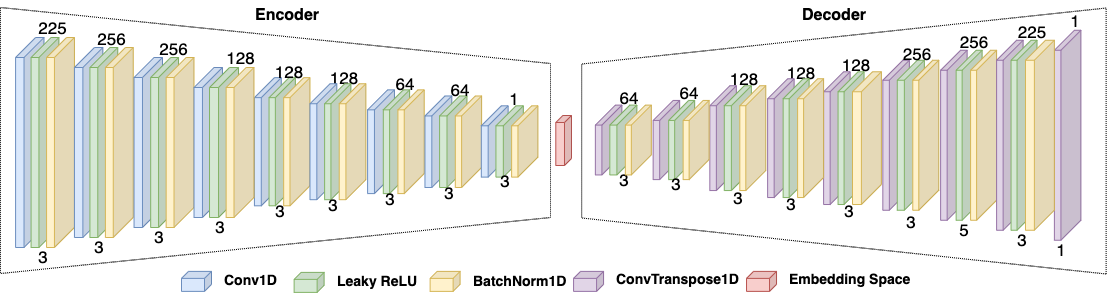
\includegraphics[width=\textwidth]{images/experiments/autoencoder_deep_1D.png}
\end{figure}



\section{Reconstruction with applied interpolation}

\section{Application of different models (configurations)}

\section{Measurement of results}